\lstset{
  basicstyle=\scriptsize\ttfamily,
  breaklines=true,
  breakatwhitespace=true,
  frame=single,
  language=TeX,
  title=\lstname
}

\makesection{Introduction}

\myframe{
  \begin{itemize}
    \item {\bf PGF} ({\bf P}ortable {\bf G}raphics {\bf F}ormat)
      é uma camada básica,
      com comandos básicos
    \item {\bf TikZ} ({\bf T}ikZ {\bf i}st {\bf k}ein {\bf Z}eichenprogramm -
      TikZ não é um programa para desenhar.)
      Uma camada {\it frontend}
      com comandos facilitando o desenho
      utilizando PGF.
    \item {\bf PGFPLOTS} Faz gráficos de alta qualidade
      usando o TikZ.
      O usuário passa informações dos eixos, e funções/dados.
  \end{itemize}
}

\makesection{TikZ}

\begin{frame}[fragile]
  \begin{verbatim}
\usepackage{tikz} % No cabeçalho

\begin{tikzpicture} % No corpo do texto
  \draw[->] (0,0) -- (1,0); % Default: cm
\end{tikzpicture}
  \end{verbatim}
  \begin{center}
  \begin{tikzpicture}
    \draw[->] (0,0) -- (1,0);
  \end{tikzpicture}
  \end{center}
\end{frame}

\myframe{
  \begin{center}
  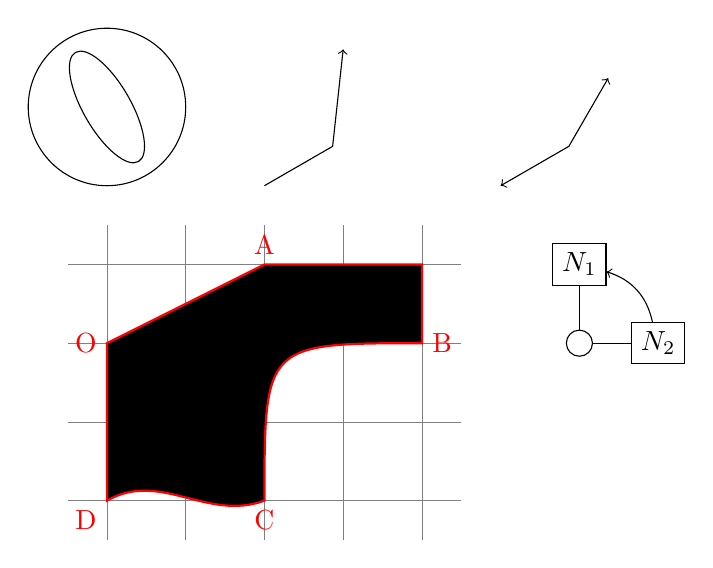
\begin{tikzpicture}
    \path[draw,->] (0,0) -- (30:1cm) -- (60:2cm);
    \draw[<->] (3,0) -- ++(30:1cm) -- ++(60:1cm);
    \draw[help lines, shift={(-2,-2)}] (-0.5,-2.5) grid (4.5,1.5);
    \path[fill,draw=red,fill=black,thick,shift={(-2,-2)}]
      (0,0) node[left,red] {O} -- (2,1) node[above,red] {A}
                          -| (4,0) node[right,red] {B}
                          .. controls (2,0) .. (2,-2) node[below,red] {C}
                          to[out=200,in=30] (0,-2) node[below left, red] {D}
                          -- cycle;
    \draw (-2,1) circle[radius=1];
    \draw (-2,1) circle[x radius=0.3, y radius=0.8, rotate=30];
    \node[draw,rectangle,black] (p1) at (4,-1) {$N_1$};
    \coordinate[draw,circle] (p2) at (4,-2);
    \node[draw,rectangle,black] (p3) at (5,-2) {$N_2$};
    \draw (p1) -- (p2) -- (p3);
    \draw[->] (p3) to[bend right] (p1);
  \end{tikzpicture}
  \end{center}
}

\begin{frame}[fragile]
  \begin{verbatim}
\path[draw,->] (0,0) -- (30:1cm) -- (60:2cm);
\draw[<->] (3,0) -- ++(30:1cm) -- ++(60:1cm);
  \end{verbatim}
  \begin{center}
  \begin{tikzpicture}
    \path[draw,->] (0,0) -- (30:1cm) -- (60:2cm);
    \draw[<->] (3,0) -- ++(30:1cm) -- ++(60:1cm);
  \end{tikzpicture}
  \end{center}
\end{frame}

\begin{frame}[fragile]
  \begin{verbatim}
\draw (0,0) circle[radius=1];
\draw (0.2,0) circle[x radius=0.3, y radius=0.8,
  rotate=30];
  \end{verbatim}
  \begin{center}
  
\begin{tikzpicture}
    \draw (0,0) circle[radius=1];
    \draw (0.2,0) circle[x radius=0.3, y radius=0.8, rotate=30];
  \end{tikzpicture}
  \end{center}
\end{frame}

\begin{frame}[fragile]
  \begin{verbatim}
\node[draw,rectangle,black] (p1) at (4,-1) {$N_1$};
\coordinate[draw,circle] (p2) at (4,-2);
\node[draw,rectangle,black] (p3) at (5,-2) {$N_2$};
\draw (p1) -- (p2) -- (p3);
\draw[->] (p3) to[bend right] (p1);
  \end{verbatim}
  \begin{center}
  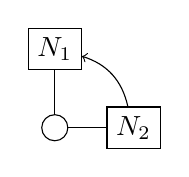
\begin{tikzpicture}
    \node[draw,rectangle,black] (p1) at (4,-1) {$N_1$};
    \coordinate[draw,circle] (p2) at (4,-2);
    \node[draw,rectangle,black] (p3) at (5,-2) {$N_2$};
    \draw (p1) -- (p2) -- (p3);
    \draw[->] (p3) to[bend right] (p1);
  \end{tikzpicture}
  \end{center}
\end{frame}

\begin{frame}[fragile]
  \scriptsize
  \begin{verbatim}
\draw[help lines, shift={(-2,-2)}] (-0.5,-2.5) grid (4.5,1.5);
\path[fill,draw=red,fill=black,thick,shift={(-2,-2)}]
  (0,0) node[left,red] {O} -- (2,1) node[above,red] {A}
    -| (4,0) node[right,red] {B}
    .. controls (2,0) .. (2,-2) node[right,red] {C}
    to[out=-30,in=210] (0,-2) node[below left, red] {D} -- cycle;
  \end{verbatim}
  \normalsize
  \begin{center}
  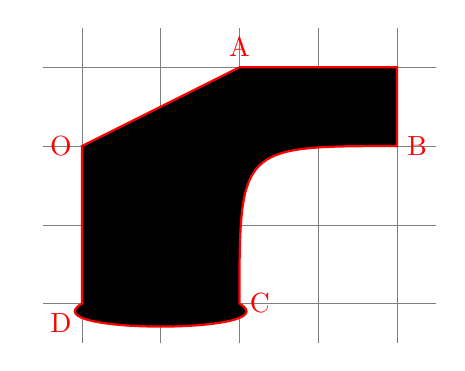
\begin{tikzpicture}
    \draw[help lines, shift={(-2,-2)}] (-0.5,-2.5) grid (4.5,1.5);
    \path[fill,draw=red,fill=black,thick,shift={(-2,-2)}]
      (0,0) node[left,red] {O} -- (2,1) node[above,red] {A}
                          -| (4,0) node[right,red] {B}
                          .. controls (2,0) .. (2,-2) node[right,red] {C}
                          to[out=-30,in=210] (0,-2) node[below left, red] {D}
                          -- cycle;
  \end{tikzpicture}
  \end{center}
\end{frame}

\begin{frame}[fragile]
  \footnotesize
  \begin{verbatim}
\draw[very thin,gray] (-0.1,-1.1) grid (4.1,4.1);
\draw[->] (-0.2,0) -- (4.2,0) node[right] {$x$};
\draw[->] (0,-1.2) -- (0,4.2) node[above] {$y$};
\draw[red]  plot(\x,{sin(\x r)}) node[right] {$f(x)=\sin x$};
\draw[blue,dashed] plot(\x,\x) node[right] {$f(x)=x$};
\draw[orange] plot(\x,{0.05*exp(\x)}) node[right] {$f(x)=0.05e^x$};
\draw[green,thick,domain=0:360]  plot({1+cos(\x)},{2.5+sin(\x)});
  \end{verbatim}
  \normalsize
\end{frame}

\begin{frame}
  \begin{center}
    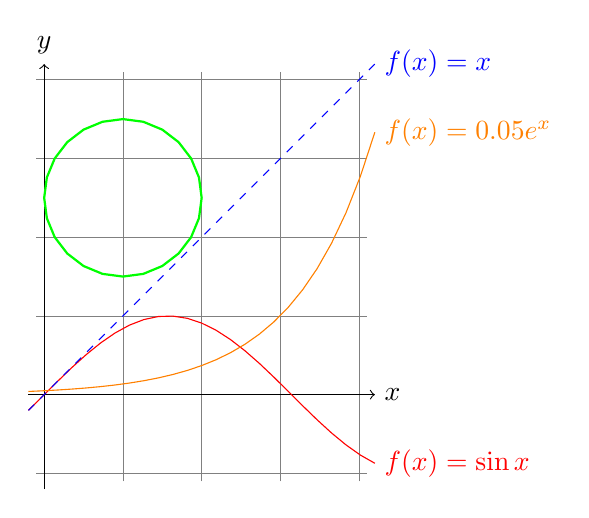
\begin{tikzpicture}[domain=-0.2:4.2]
    \draw[very thin,gray] (-0.1,-1.1) grid (4.1,4.1);
    \draw[->] (-0.2,0) -- (4.2,0) node[right] {$x$};
    \draw[->] (0,-1.2) -- (0,4.2) node[above] {$y$};
    \draw[red]  plot(\x,{sin(\x r)}) node[right] {$f(x)=\sin x$};
    \draw[blue,dashed] plot(\x,\x) node[right] {$f(x)=x$};
    \draw[orange] plot(\x,{0.05*exp(\x)}) node[right] {$f(x)=0.05e^x$};
    \draw[green,thick,domain=0:360]  plot({1+cos(\x)},{2.5+sin(\x)});
  \end{tikzpicture}
  \end{center}
\end{frame}

\begin{frame}[fragile]
  \ctr{path}
  \begin{center}
  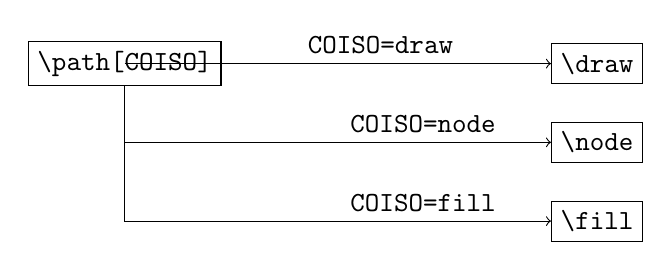
\begin{tikzpicture}
    \node[draw,rectangle] (path) at (0,0) {\verb+\path[COISO]+};
    \node[draw,rectangle] (draw) at (6,0) {\verb+\draw+};
    \node[draw,rectangle] (node) at (6,-1) {\verb+\node+};
    \node[draw,rectangle] (fill) at (6,-2) {\verb+\fill+};
    \draw[->] (path) |- (draw) node[pos=0.80,above] {\verb+COISO=draw+};
    \draw[->] (path) |- (node) node[pos=0.85,above] {\verb+COISO=node+};
    \draw[->] (path) |- (fill) node[pos=0.85,above] {\verb+COISO=fill+};
  \end{tikzpicture}
  \end{center}
\end{frame}

\begin{frame}[fragile]
  \begin{verbatim}
\draw[domain=0:1.75,red] plot (\x,{0.5*\x^2});
\foreach \x in {0.5, 0.75, ..., 1.25} {
  \draw (\x,0) -- (\x,{0.5*\x^2}) --
  ({\x+0.25},{0.5*\x^2}) -- ({\x+0.25},0) -- cycle; }
  \end{verbatim}
  \begin{center}
    \begin{tikzpicture}[scale=2]
    \draw[->] (-0.1,0) -- (2.1,0);
    \draw[->] (0,-0.1) -- (0,1.8);
    \draw[domain=0:1.75,red] plot (\x,{0.5*\x^2});
    \foreach \x in {0.5, 0.75, ..., 1.25} {
      \draw (\x,0) -- (\x,{0.5*\x^2}) -- ({\x+0.25},{0.5*\x^2}) -- ({\x+0.25},0)
      -- cycle;
    }
    \draw[blue] (0.5,0.125) -- (0.5,0) node[below] {$a$};
    \draw[blue] (1.5,1.125) -- (1.5,0) node[below] {$b$};
  \end{tikzpicture}
  \end{center}
\end{frame}

\begin{frame}[fragile]
  \ctr{Beamer}
  \begin{verbatim}
\only<1>{A}
\onslide<2>{B}
\only<2-3>{C}
  \end{verbatim}
\only<1>{A}
\onslide<2>{B}
\only<2-3>{C}
\end{frame}

\begin{frame}[fragile]
\begin{verbatim}
\usetikzlibrary{patterns}
\draw (0,0) rectangle (4,4);
\onslide<2->{\draw[pattern=dots] (0,0) rectangle (2,2);}
\only<3->{\draw[pattern=dots] (2,2) rectangle (3,3);}
\only<4->{\draw[pattern=dots] (3,3) rectangle
  (3.5,3.5);}
\only<5->{\draw[pattern=dots] (3.5,3.5) rectangle
  (3.75,3.75);}
\only<6->{\draw[pattern=dots] (3.75,3.75) rectangle
  (3.875,3.875);}
\end{verbatim}
\end{frame}

\usetikzlibrary{patterns}
\frame{
  \begin{center}
    \begin{tikzpicture}
    \draw (0,0) rectangle (4,4);
    \onslide<2->{\draw[pattern=dots] (0,0) rectangle (2,2);}
    \only<3->{\draw[pattern=dots] (2,2) rectangle (3,3);}
    \only<4->{\draw[pattern=dots] (3,3) rectangle (3.5,3.5);}
  \end{tikzpicture}
  \end{center}
}

\begin{frame}[fragile]
  \begin{verbatim}
\draw (0,0) rectangle (4,4);
\foreach \n in {1,...,4} {
  \only<\n->{
    \def\a{{4-2^(3-\n)}}
    \def\b{{4-2^(2-\n)}}
    \draw[blue,fill]
      (\a,\a) rectangle (\b,\b);
  }
}
  \end{verbatim}
\end{frame}

\frame{
  \begin{center}
    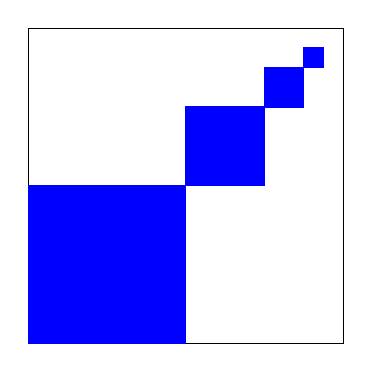
\begin{tikzpicture}
    \draw (0,0) rectangle (4,4);
    \foreach \n in {1,...,4} {
      \only<\n->{
        \def\a{{4-2^(3-\n)}}
        \def\b{{4-2^(2-\n)}}
        \draw[blue,fill]
          (\a,\a) rectangle (\b,\b);
      }
    }
  \end{tikzpicture}
  \end{center}
}

\frame{
  \begin{itemize}
    \item Grafos
    \item Árvores
    \item Fluxogramas
    \item Funções
  \end{itemize}
}

\makesection{PgfPlots}

\begin{frame}[fragile]
  \lstinputlisting[firstline=7]{pgfplots-ex1.tex}
\end{frame}

\frame{
  \begin{center}
    \includegraphics[height=0.95\textheight]{pgfplots-ex1.pdf}
  \end{center}
}

\begin{frame}[fragile]
  \lstinputlisting[firstline=7]{pgfplots-ex2.tex}
\end{frame}

\frame{
  \begin{center}
    \includegraphics[height=0.95\textheight]{pgfplots-ex2.pdf}
  \end{center}
}

\begin{frame}[fragile]
  \lstinputlisting[firstline=7]{pgfplots-ex3.tex}
\end{frame}

\frame{
  \begin{center}
    \includegraphics[height=0.95\textheight]{pgfplots-ex3.pdf}
  \end{center}
}

\frame{
  \includegraphics[width=0.49\textwidth]{filtro-fh.pdf}
  \includegraphics[width=0.49\textwidth]{filtro.pdf}
}

\begin{frame}[fragile,allowframebreaks]
  \lstinputlisting[
      firstline=14
    ]{filtro.tex}
\end{frame}

\frame{
  \lstinputlisting[firstline=7]{mountain.tex}
  \lstinputlisting[lastline=3, frame=single]{dados/data.dat}
}

\frame{
  \begin{center}
    \includegraphics[height=0.8\textheight]{mountain.pdf}
  \end{center}
}

\frame{
  \begin{center}
    \includegraphics[height=0.8\textheight]{mountain-cm.pdf}
  \end{center}
}
